%%%%%%%%%%%%%%%%%%%%%%%%%%%%%%%%%%%%%%%%%
% Dreuw & Deselaer's Poster
% LaTeX Template
% Version 1.0 (11/04/13)
%
% Created by:
% Philippe Dreuw and Thomas Deselaers
% http://www-i6.informatik.rwth-aachen.de/~dreuw/latexbeamerposter.php
%
% This template has been downloaded from:
% http://www.LaTeXTemplates.com
%
% License:
% CC BY-NC-SA 3.0 (http://creativecommons.org/licenses/by-nc-sa/3.0/)
%
%%%%%%%%%%%%%%%%%%%%%%%%%%%%%%%%%%%%%%%%%

%----------------------------------------------------------------------------------------
%	PACKAGES AND OTHER DOCUMENT CONFIGURATIONS
%----------------------------------------------------------------------------------------

\documentclass[final,hyperref={pdfpagelabels=false}]{beamer}

\usepackage[orientation=portrait,size=a1]{beamerposter} % Use the beamerposter package for laying out the poster with a portrait orientation and an a0 paper size

\usetheme{I6pd2} % Use the I6pd2 theme supplied with this template

\usepackage[english]{babel} % English language/hyphenation

\usepackage{amsmath,amsthm,amssymb,latexsym} % For including math equations, theorems, symbols, etc

%\usepackage{times}\usefonttheme{professionalfonts}  % Uncomment to use Times as the main font
%\usefonttheme[onlymath]{serif} % Uncomment to use a Serif font within math environments

\boldmath % Use bold for everything within the math environment

\usepackage{booktabs} % Top and bottom rules for tables

\graphicspath{{figures/}} % Location of the graphics files

\usepackage{subfigure}
\usepackage{xeCJK}
	\setCJKmainfont{cwTeX Q HeiZH}

\usecaptiontemplate{\small\structure{\insertcaptionname~\insertcaptionnumber: }\insertcaption} % A fix for figure numbering

%----------------------------------------------------------------------------------------
%	TITLE SECTION 
%----------------------------------------------------------------------------------------

\title{\huge So, Where Are the Ads?} % Poster title

\author{B02705008 江昱熹、B02902056 江韋霖、B02902034 邱筱晴、B02705019陳姿穎} % Author(s)

\institute{Computer Science and Information Engineering, National Taiwan University } % Institution(s)

%----------------------------------------------------------------------------------------
%	FOOTER TEXT
%----------------------------------------------------------------------------------------

\newcommand{\leftfoot}{} % Left footer text

\newcommand{\rightfoot}{} % Right footer text

%----------------------------------------------------------------------------------------

\begin{document}

\addtobeamertemplate{block end}{}{\vspace*{2ex}} % White space under blocks

\begin{frame}[t] % The whole poster is enclosed in one beamer frame

\begin{columns}[t] % The whole poster consists of two major columns, each of which can be subdivided further with another \begin{columns} block - the [t] argument aligns each column's content to the top

\begin{column}{.02\textwidth}\end{column} % Empty spacer column

\begin{column}{.465\textwidth} % The first column


%----------------------------------------------------------------------------------------
%	INTRODUCTION
%----------------------------------------------------------------------------------------
            
\begin{block}{Introduction}

\par Instagram is an online mobile photo-sharing, video-sharing and social networking service, which rapidly gained popularity, with over 300 million as of December 2014. One of the features in Instagram is that users can add hashtags on their posts. Using specific tags help users connect with other like-minded people on Instagram. For example, when searching \#cat on Instagram, users can explore a veriaty of photos related to cats. 

\quad Therefore, we wonder how well do the Chinese hashtags perform on Instagram. We searched for posts with hashtag \#台灣. Out of our expectation, instead of geting beautiful scenes in Taiwan or anything related, the results were full of spamming and advertising posts! That’s a bad user-experience. Therefore, we decided to imporve the quility of results when searching for Chinese hashtags through recognizing the spam posts with machine learning techniques.
 
\begin{figure}
\centering
\subfigure[A normal post in \#台灣]{
	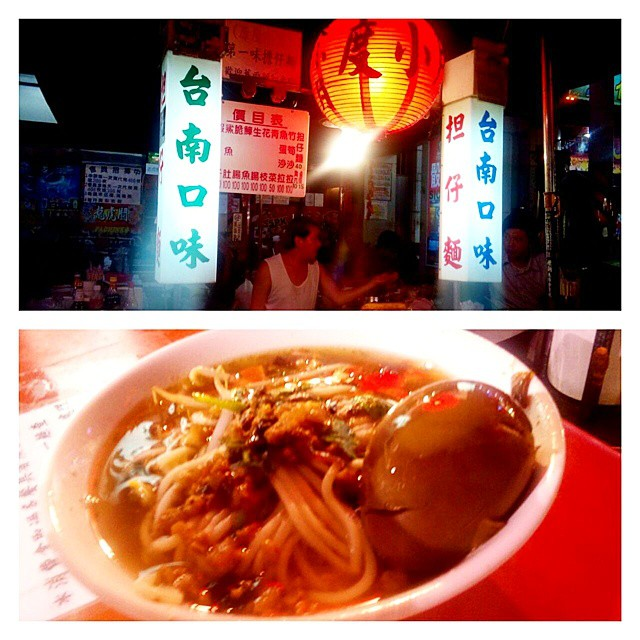
\includegraphics[width=0.25\linewidth]{normpost.jpg}
}
\hspace{1em}
\subfigure[A spam post in \#台灣]{
	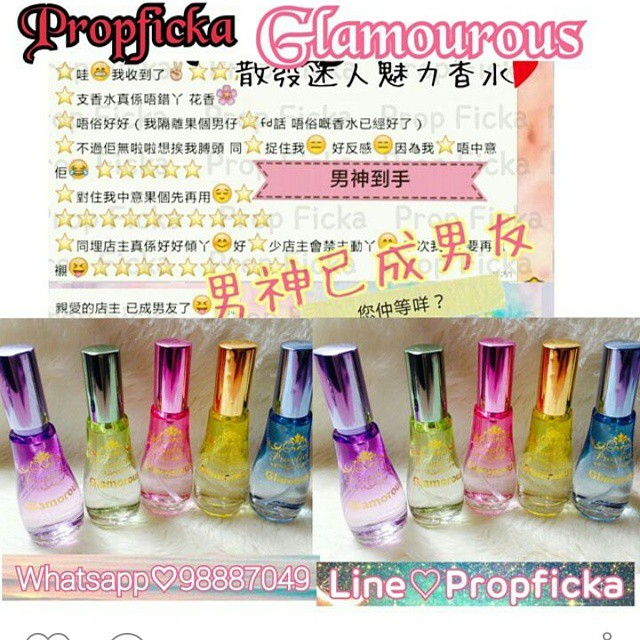
\includegraphics[width=0.25\linewidth]{spampost.jpg}
}
\end{figure}


\end{block}

%----------------------------------------------------------------------------------------
%	MATERIALS
%----------------------------------------------------------------------------------------

\begin{block}{Workflow}

%\begin{columns} % Subdivide the first main column
%\begin{column}{.54\textwidth} % The first subdivided column %within the first main column
%\begin{itemize}
%\item Vestibulum nisl, quis euismod velit eros in ligula.
%\begin{itemize}
%\item Cras rhoncus quam et augue convallis in elementum urna %tincidunt.
%\end{itemize}
%\item Proin ut vestibulum augue.
%\begin{itemize}
%\item Donec dapibus sagittis neque eu ultrices.
%\end{itemize}
%\end{itemize}
%\end{column}

%\begin{column}{.43\textwidth} % The second subdivided column within the first main column

First, we collect many posts with different hashtags from Instagram. Then classify whether a post is spamming manually by a tool we write. After classifying posts, we divide the data into two parts of same size, which correspond to training data and testing data. In training data, we try hard to observe some features in spam posts and come up with some measurable properties, which we will discuss the result detailly in Section Model. In Section Method, we will compare the performance of some popular machine learning techniques with different features selection. Finally, our ultimate goal is to provide a useful web application for users. 

\centering
\begin{figure}
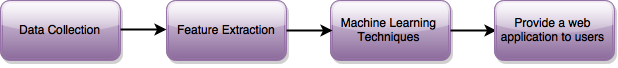
\includegraphics[scale=1]{workflow.png}
\caption{Workflow of the project.}
\end{figure}
%\end{column}
%\end{columns} % End of the subdivision


\end{block}

%----------------------------------------------------------------------------------------
%	OBSERVATION AND FEATURE EXTRACTION
%----------------------------------------------------------------------------------------

\begin{block}{Observation and Feature Extraction}



%\begin{description}
\begin{tabular}{ll}
Digits & Advertisers often need to provide the contact way, such as phone numbers. \\
Hashtags & Advertisers usually use many tags to let the post easily appear in search results. \\
Social media & Advertisers sometimes will provide social accounts such as Line, whatsapp, Facebook, etc. \\
Keywords & We try to find the keywords which advertisers often use in posts by some analysis.

\end{tabular}

\end{block}


%----------------------------------------------------------------------------------------
%	Feature Sets Details
%----------------------------------------------------------------------------------------

\begin{block}{Feature Sets Details}

\begin{itemize}
\item Feature Set 1 -- Naive Features
	\begin{itemize}
		\item First, we come up with simple features, including \texttt{tag-amount}, \texttt{longest-digits}, \texttt{social-media}, \texttt{keyword-count}, \texttt{like-amount}, \texttt{comment-amount}, \texttt{follower-amount}, \texttt{post-amount-5day}, ...etc., totally 11 features. In particular, we only consider nine keywords when calculating keyword. Notice that we consider not only the content in posts, but also in author profile.  
	\end{itemize}
\item Feature Set 2 -- Unigram Language Model
	\begin{itemize}
		\item To strengthen the model, we analyize the training data with \texttt{Jieba}, a Chinese text segmentation tool. With \texttt{Jieba}, we calculate the frequency of each word and each single character. Then, select those occur more than 50 times as feature with its time of appearance as value. Eventually, 1113 features in total.
	\end{itemize}
\end{itemize}


%\begin{itemize}
%\item Feature Set 1
%	\begin{itemize}
%		\item Based on the observation above, we come up with some simple features at first, which includes \texttt{tag-amount}, \texttt{longest-digits}, \texttt{social-media}, \texttt{keyword-count}, \texttt{like-amount}, \texttt{comment-amount}, \texttt{follower-amount}, \texttt{post-amount-5day} ..., totally 11 features. In particular \texttt{keyword-count}, we only consider about ten words produced by us. Notice that we consider not only the content in posts, but also the info page of authors. We think that makes sense since advertisers usually put the contact info to author description. 
%	\end{itemize}
%\item Feature Set 2
%	\begin{itemize}
%		\item However, it is not enough to become a general model by using only ten keywords. Therefore, we take some analysis on the training data by a Chinese text segmentation tool called \texttt{jieba}. By using the tool, we count frequency of each word and select the ones occur more than 50 times, and then pick the words as the features, representing how many times the words appear in contents. The method actually called uni-gram in Language Model. Similarly, we also take Chinese character into consideration, and finally the number of features will up to 1113.
%	\end{itemize}
%\end{itemize}
\end{block}



%----------------------------------------------------------------------------------------
%	Data Description
%----------------------------------------------------------------------------------------

\begin{block}{Data Description}

We randomly split the hashtags into two parts with same posts size 960. Note that we do not random by posts but by hashtags, since we want to examine whether our model would still perform well on different hashtags.

\begin{table}[h]
\centering

\label{data-table}
\begin{tabular}{lll}
\multicolumn{1}{l|}{Hashtags (top - training data, bottom - testing data)}                                                                                 & \multicolumn{1}{l|}{spam} & not spam \\ \hline
\multicolumn{1}{l|}{\begin{tabular}[c]{@{}l@{}}文青、日本、母親節、吃飯、龍貓、早安、蔬菜、都敏俊\\ 蛋黃哥、夏天、五月天、運動、髮型、馬卡龍、台灣、正妹\end{tabular}} & \multicolumn{1}{l|}{417}  & 543      \\ \hline
\multicolumn{1}{l|}{\begin{tabular}[c]{@{}l@{}}天氣、哭、可愛、人生、廢話、香港、生日快樂、羊駝\\ 迪士尼、夜景、閃光、美食、腳踏車、海邊、北海道、貓咪\end{tabular}}  & \multicolumn{1}{l|}{726}  & 234      
                                                                                                                    
\end{tabular}
\caption{Total 1920 posts, in which a hashtag consist of 60 posts.}
\end{table}



\end{block}

%----------------------------------------------------------------------------------------
%	DEMO
%----------------------------------------------------------------------------------------

\begin{block}{Website Demo}

\begin{columns}

\begin{column}{.5\textwidth}

\begin{figure}
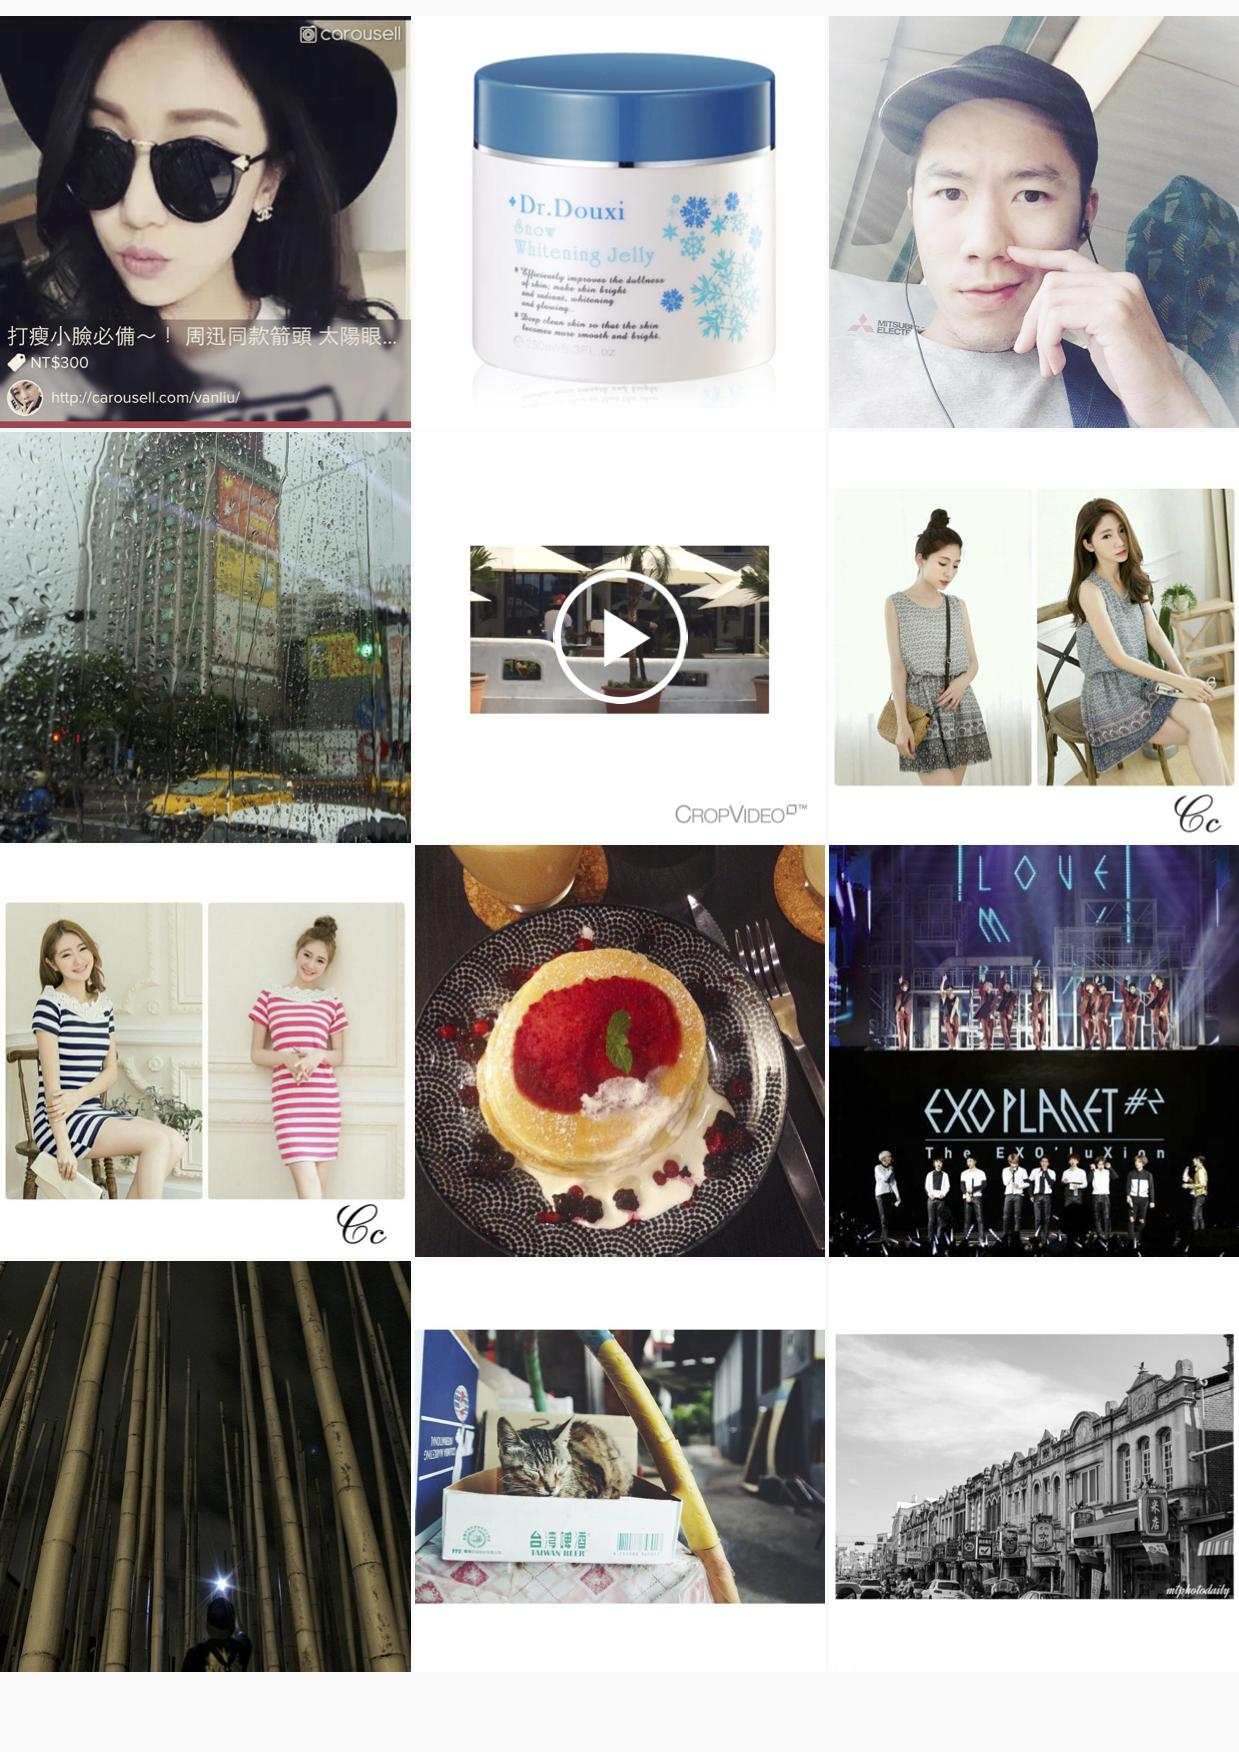
\includegraphics[width=0.75\linewidth]{before}
\caption{search \#台灣 on Instagram}
\end{figure}

\end{column}

\begin{column}{.5\textwidth}

\begin{figure}
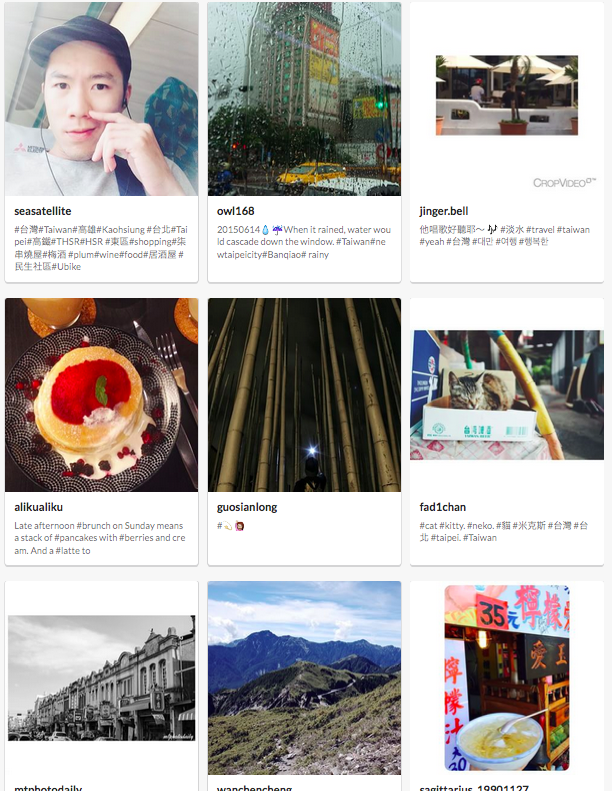
\includegraphics[width=0.8\linewidth]{after}
\caption{search \#台灣 on our website}
\end{figure}

\end{column}

\end{columns}

\end{block}


%\begin{block}{Method}

%\begin{columns}

%\begin{column}{.5\textwidth}
%\begin{itemize}

%\item \texttt{Decision Tree} \\
	%\begin{itemize}
	%	\item 
		%Decision tree is a classification algorithm that performs a recursive binary partitioning of the feature space. The tree predicts the same label for each leaf partition. Each partition is chosen by selecting the best split from a set of possible splits, in order to maximize the information gain at a tree node. Here we  use the implementation in \texttt{scikit-learn}\cite{scikit-learn} library.
	%\end{itemize}
%\end{itemize}

%\end{column}

%\begin{column}{.4\textwidth}

%\begin{figure}
%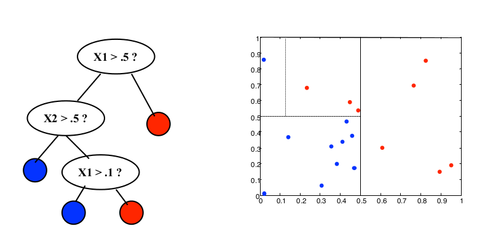
\includegraphics[width=1\linewidth]{decision_tree.png}
%\caption{Decision tree}
%\end{figure}

%\end{column}

%\end{columns}

%\end{block}

%----------------------------------------------------------------------------------------

\end{column} % End of the first column

\begin{column}{.03\textwidth}\end{column} % Empty spacer column
 
\begin{column}{.465\textwidth} % The second column

%----------------------------------------------------------------------------------------
%	METHOD
%----------------------------------------------------------------------------------------

\begin{block}{Method}

\begin{columns}

\begin{column}{.5\textwidth}
\begin{itemize}

\item \texttt{Decision Tree} \\
	\begin{itemize}
		\item 
		Decision tree is a classification algorithm that performs a recursive binary partitioning of the feature space. The tree predicts the same label for each leaf partition. Each partition is chosen by selecting the best split from a set of possible splits, in order to maximize the information gain at a tree node. Here we  use the implementation in \texttt{scikit-learn} \cite{scikit-learn} library.
	\end{itemize}
\item \texttt{Random Forests} \\
	\begin{itemize}
		\item In Random Forests, each tree in the ensemble is built from a sample subset from the features. That is, when splitting a node during the construction of the tree, the split that is chosen is no longer the best split among all features. Instead, the split that is picked is the best split among a random subset of the features. Here we use the implementation in \texttt{scikit-learn} library.
	\end{itemize}


	
	
\item \texttt{Support Vector Machines} \\
\begin{itemize}
\item A support vector machine constructs a hyperplane or set of hyperplanes in a high dimensional space, which can be used for classification, regression. Intuitively, a good separation is achieved by the hyperplane that has the largest distance to the nearest training-data point of any class (so-called functional margin), since in general the larger the margin the lower the generalization error of the classifier. Here we use the popular software \texttt{liblinear}\cite{REF08a} and \texttt{libsvm}\cite{CC01a}.
\end{itemize}
	
\end{itemize}

\end{column}

\begin{column}{.4\textwidth}

\begin{figure}
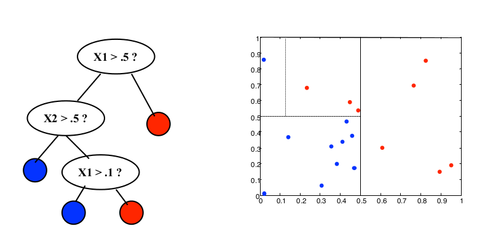
\includegraphics[width=1\linewidth]{decision_tree.png}
\caption{Decision tree}
\end{figure}

\begin{figure}
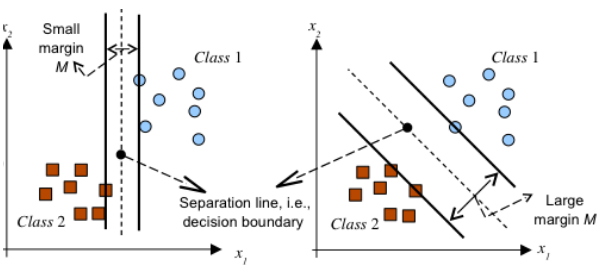
\includegraphics[width=1\linewidth]{svm-core.png}
\caption{Maximal margin hyperplane}
\end{figure}


\begin{figure}
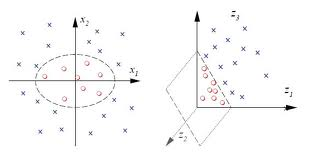
\includegraphics[width=1\linewidth]{kernel-trick.jpeg}
\caption{Kernel support vector machine}
\end{figure}


\end{column}

\end{columns}

     
\end{block}

%------------------------------------------------

\begin{block}{Results}

To our surprise, the performance of every method are amazing. We think the reason is that we get the important features in spam posts. By applying some feature selection tools\cite{YW04a}, we discover that \texttt{longest-digits}, \texttt{total-digits}, \texttt{tag-amount} is the most critical features we have. We can only use five features to perform high prediction(about 95\%). 

\begin{table}[h]
\centering
\caption{Results of using default settings on each method}
\label{result1}
\begin{tabular}{l|l|l}
                    & Testing Accuracy on Set 1     & Testing Accuracy on Set 2     \\ \hline
\texttt{Decision Tree}       & 94.58\% (908/960) & 93.33\% (896/960) \\ \hline
\texttt{Random Forests}      & 95.94\% (921/960) & 96.56\% (927/960) \\ \hline
\texttt{linear SVM (l2\_l2)} & 91.56\% (879/960) & 91.86\% (882/960) \\ \hline
\texttt{RBF Kernel SVM (c-SVC)}      & 76.35\% (733/960) & 85.21\% (818/960)        
\end{tabular}
\end{table}

Another point is that \texttt{Kernel SVM} performs bad in the default settings. The reason is that we do not scale data before applying SVM, which will lead to features with greater numeric ranges dominate those in smaller numeric ranges. After scaling data, the performance dramatically improved, check the results in Table \ref{result2}. Also, the parameter selection on SVM is important. Here we use 5-fold cross validation to select parameter $C$ \cite{BYC15a} and ($\gamma$ in \texttt{Kernel SVM}), which also improve the performance on testing data.


\begin{table}[h]
\centering
\caption{Compare scaling data and parameter selection by using 5-fold cross validation on SVMs}
\label{result2}
\begin{tabular}{l|l|l}
                                           & Testing Accuracy on Set 1 & Testing Accuracy on Set 2 \\ \hline
\texttt{linear SVM} (scaled data)                & 97.92\% (940/960)         & 97.08\% (932/960)         \\ \hline
\texttt{linear SVM} (5-fold CV) & 98.02\% (941/960)         & 97.97\% (940/960)         \\ \hline
\texttt{kernel SVM} (scaled data)                & 96.7708\% (929/960)       & 93.54\% (898/960)         \\ \hline
\texttt{kernel SVM} (5-fold CV) & 98.2292\% (943/960)       & 97.29\% (934/960)                        
\end{tabular}
\end{table}

\end{block}

%----------------------------------------------------------------------------------------
%	DEMO
%----------------------------------------------------------------------------------------

%\begin{block}{Website Demo}

%begin{columns}

%\begin{column}{.4\textwidth}

%\begin{figure}
%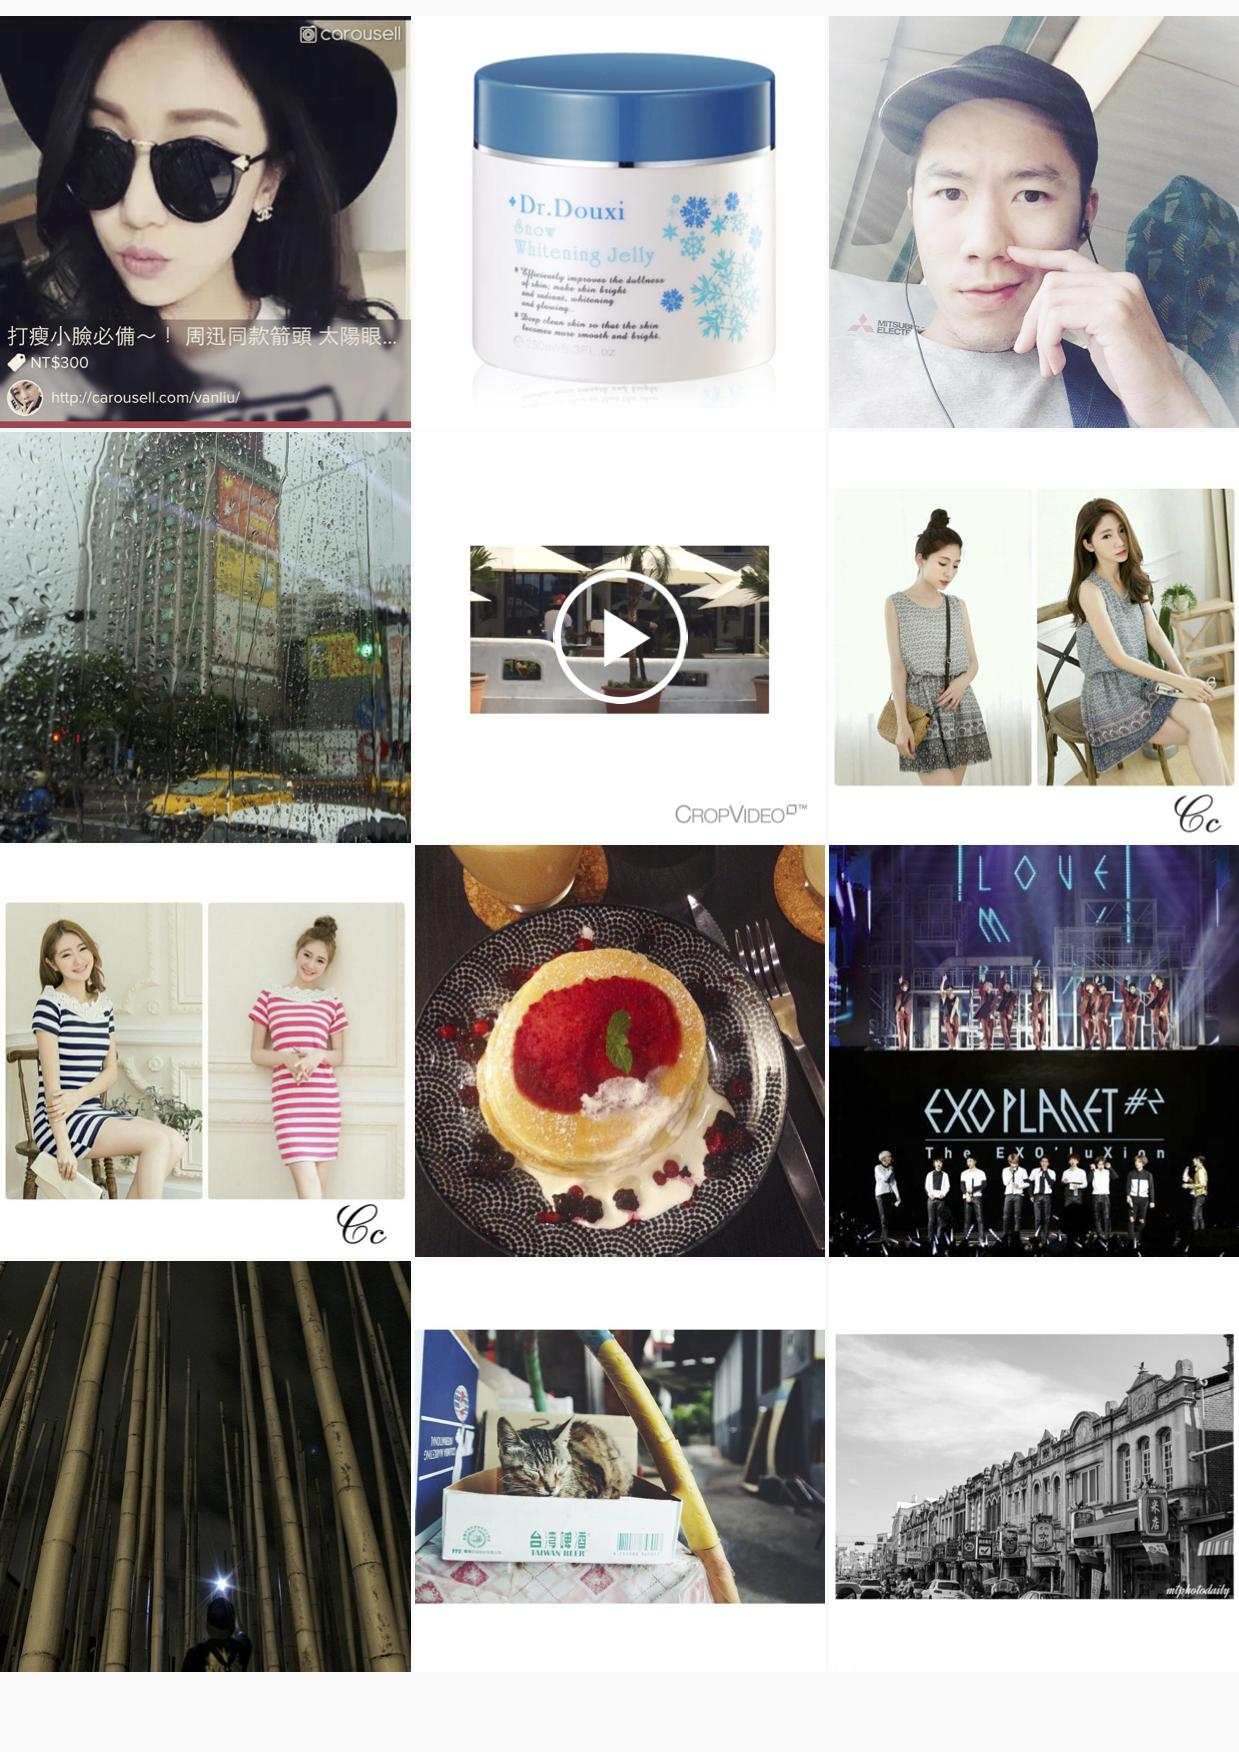
\includegraphics[width=0.75\linewidth]{before}
%\caption{Before}
%\end{figure}

%\end{column}

%\begin{column}{.4\textwidth}

%\begin{figure}
%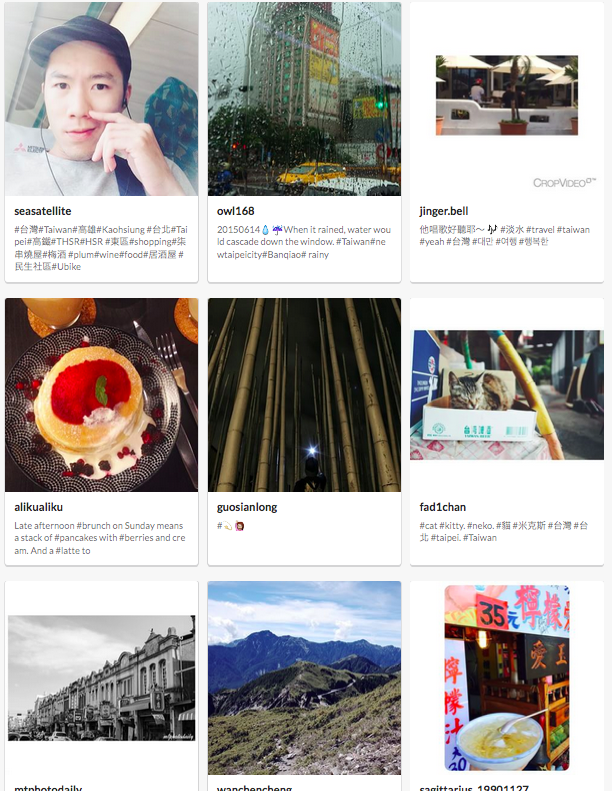
\includegraphics[width=0.8\linewidth]{after}
%\caption{After}
%\end{figure}

%\end{column}

%\end{columns}

%\end{block}


%----------------------------------------------------------------------------------------
%	CONCLUSION
%----------------------------------------------------------------------------------------

\begin{block}{Conclusion and Future Works}

Though our current model has performed well on the testing data, there are still some improvements can be done. First, in our current model, we only count the times of keywords appearance, regardless of the order of words. Thus, to make the model more precise, we may apply Natural Language Processing(NLP) methods to analyze the semantics of a post. 

\quad Secondly, there are information lying in the pictures that we ignore in our model. Some adveritsers tend to show selling information on their sharing-photos, including the price of products, social accounts and so on. We may use the Optical Character Recognition (OCR) techniques to extract these features. Besides characters, recognizing the objects in the pictures helps as well. We have discovered some auto-tagging APIs such as \texttt{imagga.com} and \texttt{JARVIS.ai}. These APIs are able to tell the possible concepts of a given image. We will apply them to improve the prediction, or even build a Convolutional Neural Network by ourself to accomplish the image recognition.

%Third, we want to improve the performance of our web server. While browsing the current website, delay may occur when scrolling down since the server has to fetch the author’s recent posts, bio, etc. for each request. One possible way to fix the problem is adding cache, thus we don’t have to fetch the same contents twice.

\end{block}

%----------------------------------------------------------------------------------------
%	REFERENCES
%----------------------------------------------------------------------------------------

\begin{block}{References}

%\nocite{*} % Insert publications even if they are not cited in the poster
\bibliographystyle{ieeetr}
\bibliography{sample}

\end{block}


%----------------------------------------------------------------------------------------

\end{column} % End of the second column

\begin{column}{.015\textwidth}\end{column} % Empty spacer column

\end{columns} % End of all the columns in the poster

\end{frame} % End of the enclosing frame

\end{document}